%\RequirePackage{snapshot}
\documentclass[a4paper,KOMA,landscape]{powersem}
\usepackage[display,stmo]{ifmslide}
\usepackage{soul}
%\usepackage[dvips]{graphicx}
%% user definitions
\newcommand{\ifmslide}{{\code{ifmslide.sty}}}
\newcommand{\tp}{{\code{texpower{}} \cite{texpower} }}
\newcommand{\hf}{{\code{hyperref{}} \cite{hyperref} }}
\hypersetup{pdfauthor={Henrik Frisk and Stefan �stersj�}}
\hypersetup{pdftitle={Negotiating the Musical Work. \\An empirical study on the
inter-relation between composition, interpretation and performance.}}
\hypersetup{pdfsubject={presentation}}
\hypersetup{bookmarksopen={false}}
\hypersetup{pdfpagemode={None}}

\IfFileExists{cmtt.sty}{\usepackage[override]{cmtt}%
                        \newcommand{\bs}{{\mtt\\}}}{%
                        \newcommand{\bs}{{$\setminus$}}}%

\panelposition{bottom}
\panellogo{Ulomacvnege}
\releaselogo
\freelogo(190,135)[5cm]

%%%%%%%%%%%%%%%%%%%%%%%%%%%%%%%%%%%%%%%%%%%%%%%%%%%%%%%%%%%%%%%%%%%%
%\usepackage{thumbpdf}
%%%%%%%%%%%%%%%%%%%%%%%%%%%%%%%%%%%%%%%%%%%%%%%%%%%%%%%%%%%%%%%%%%%%
\begin{document}
\headskip=12mm
\sffamily

\orgname{Malm\"{o} Academy of Music - Lund University}

\title{\begin{minipage}[t]{0.98\textwidth}\begin{center}
      {\mdseries Negotiating the musical work. \\Computer-Performer interaction in relation to Composer-Performer
interaction.\\}
\vspace{1cm}
     {\mdseries DTPA 2006}
    \end{center}\end{minipage}}

\author{\scalebox{1}[1.3]{Henrik Frisk \& Stefan \"{O}stersj\"{o}}}

\address{\href{mailto:henrik.frisk@mhm.lu.se}
  {henrik.frisk@mhm.lu.se} \href{mailto:stefan\_ostersjo@hotmail.com}{stefan\_ostersjo@hotmail.com}}
%\orgurl{http://www.henrikfrisk.com}
\slidepagestyle{panel}
%%%%%%%%%%%%%%%%%%%%%%%%%%%%%%%%%%%%%%%%%%%%%%%%%%%%%%%%%%%%%%%%%%%%
\begin{slide}
 \maketitle
\end{slide}
%%%%%%%%%%%%%%%%%%%%%%%%%%%%%%%%%%%%%%%%%%%%%%%%%%%%%%%%%%%%%%%%%%%%
\centerslidesfalse
\begin{slide}
  \section{Overview}
  \pause
  \liststepwise
      {
        \begin{itemize}
	 \item{Pre-study for a new work for guitar and computer - }
	 \step{\item{a study of the inter-relations between composer and performer.}}
	 \step{\item{Analysis of a video recording of a
	      composer/performer session.}}
	 \step{\item{Discussion of computer-performer interaction.}}
	 \step{\item{Summary}}
         \end{itemize}
      }
\end{slide}
%%%%%%%%%%%%%%%%%%%%%%%%%%%%%%%%%%%%%%%%%%%%%%%%%%%%%%%%%%%%%%%%%%%%

%%%%%%%%%%%%%%%%%%%%%%%%%%%%%%%%%%%%%%%%%%%%%%%%%%%%%%%%%%%%%%%%%%%%
\begin{slide}
  \section{Introduction}
  \subsection*{Purpose and Conditions}
  \pause
  \liststepwise
      {
        \begin{itemize}
	 \item{The musical work before its ultimate notation and performance.}
	 \step{\item{Mixed media music.}}
	 \step{\item{Wish to gain a deeper understanding of the
	      underlying processes in the communication between the
	      composer and the performer.}}
	 \step{\item{Making use of this knowledge when constructing
	      interactive performance systems.}}
	 \step{\item{Conditions.}}
        \end{itemize}
      }
\end{slide}
%%%%%%%%%%%%%%%%%%%%%%%%%%%%%%%%%%%%%%%%%%%%%%%%%%%%%%%%%%%%%%%%%%%%

%%%%%%%%%%%%%%%%%%%%%%%%%%%%%%%%%%%%%%%%%%%%%%%%%%%%%%%%%%%%%%%%%%%%
\begin{slide}
 \section{Construction - Reproduction\\/ Composer - Performer}
      \liststepwise
      {

      \step
            {
	    Traditional view\\

              \begin{minipage}[h]{\textwidth}\begin{center}
                  {\includegraphics[width=0.9\textwidth]{img/cons-rep.pdf}} \end{center}
              \end{minipage}
            }
      }
\end{slide}
%%%%%%%%%%%%%%%%%%%%%%%%%%%%%%%%%%%%%%%%%%%%%%%%%%%%%%%%%%%%%%%%%%%%

%%%%%%%%%%%%%%%%%%%%%%%%%%%%%%%%%%%%%%%%%%%%%%%%%%%%%%%%%%%%%%%%%%%%
\begin{slide}
 \section*{Construction - Reproduction\\/ Composer - Performer}
	    Ric{\oe}ur

              \begin{minipage}[h]{\textwidth}\begin{center}
                  {\includegraphics[width=0.9\textwidth]{img/cons-rep-ricoeur.pdf}} \end{center}
              \end{minipage}
\end{slide}
%%%%%%%%%%%%%%%%%%%%%%%%%%%%%%%%%%%%%%%%%%%%%%%%%%%%%%%%%%%%%%%%%%%%

%%%%%%%%%%%%%%%%%%%%%%%%%%%%%%%%%%%%%%%%%%%%%%%%%%%%%%%%%%%%%%%%%%%%
\begin{slide}
  \section{Semiological approach.}
  \liststepwise { 

  \step{\subsection*{Musical semiology}
  \begin{itemize}
   \item {Analytical understanding of the musical work in its entirety.}
  \end{itemize}
  }

  \step{\subsection*{Background to musical semiology}}
  \step{{\small {\itshape The notion of a 'single, well-defined item of information
      to be transmitted, all the rest being simply noise' is
      'dangerously inaccurate and misleading as soon as we move from the
      artificial communication of information to a concrete act of human
      communication as a total social fact.'}} \cite{molino}}  
      
      \step{{\small  Duchamp: {\itshape two poles, the artist and the viewer. The intention of
      the artist holds no significance to the viewer.}}}

      \step{{\small Val\'{e}ry: {\itshape 'there is no guarantee of a direct
      correspondance between the effect produced by a work of art and the
      intentions of its creator'.}}} 
}
\end{slide}
%%%%%%%%%%%%%%%%%%%%%%%%%%%%%%%%%%%%%%%%%%%%%%%%%%%%%%%%%%%%%%%%%%%%

%%%%%%%%%%%%%%%%%%%%%%%%%%%%%%%%%%%%%%%%%%%%%%%%%%%%%%%%%%%%%%%%%%%%
\begin{slide}
  \section{The three dimensions}
  \liststepwise { 

  \step{...recognizing, elaborating, and articulating the three relatively
autonomous levels (poietic, neutral and esthesic) facilitates
knowledge of all processes unleashed by the musical work, from the
moment of the work's conception, passing through its 'writing down',
to its performance. \cite{nattiez}}  

       \step{A model of analysis on three levels:}
          \step
              {
                \begin{itemize}
		 \item{the poietic - the constructive phase}
                  \step{\item{the esthesic - the interpretative phase}}
                  \step{\item{the neutral - the trace}}
                \end{itemize}
              }
}
\end{slide}
%%%%%%%%%%%%%%%%%%%%%%%%%%%%%%%%%%%%%%%%%%%%%%%%%%%%%%%%%%%%%%%%%%%%

%%%%%%%%%%%%%%%%%%%%%%%%%%%%%%%%%%%%%%%%%%%%%%%%%%%%%%%%%%%%%%%%%%%%
\begin{slide}
 \section{Method}
  \liststepwise {
  
  \step {\subsection*{Musical semiology.}

  Drawing on Nattiez and Molino and their idea of tripartition.
  }

  \step {\subsection*{Qualitative research.}

  Using a qualitative method when approaching the complex area of
  machine-musician interaction.
  }

  \step {\subsection*{Verbatim transcription of the video.}

  Doing a verbatim transcription of video documentation from which a graph
  was extracted.
  }
%  {
%  \begin{itemize}
%   \item{\subsection*{Musical semiology.}} 
%   \step{\item {\subsection*{Qualitative research.}}}
%   \step{\item {\subsection*{Verbatim transcription of the video.}}}
%  \end{itemize}
%  }
   }
\end{slide}
%%%%%%%%%%%%%%%%%%%%%%%%%%%%%%%%%%%%%%%%%%%%%%%%%%%%%%%%%%%%%%%%%%%%

%%%%%%%%%%%%%%%%%%%%%%%%%%%%%%%%%%%%%%%%%%%%%%%%%%%%%%%%%%%%%%%%%%%%
\begin{slide}
  \section{Example page of transcription.}
              \begin{minipage}[h]{\textwidth}
	       \begin{center}
	       {\includegraphics[width=0.75\textwidth]{img/transcription.pdf}} 
	       \end{center}
              \end{minipage}
\end{slide}
%%%%%%%%%%%%%%%%%%%%%%%%%%%%%%%%%%%%%%%%%%%%%%%%%%%%%%%%%%%%%%%%%%%%

%%%%%%%%%%%%%%%%%%%%%%%%%%%%%%%%%%%%%%%%%%%%%%%%%%%%%%%%%%%%%%%%%%%%
\begin{slide}
  \section{Empirical study}
  \liststepwise { 

  \subsection*{background}

  \step{
  \begin{itemize}
   \item {Love Mangs: Viken for guitar, banjo, e-bow and electronics
	 (2004-05).}
   \step{\item {Video documentation of a working session with guitarist Stefan
	 \"{O}stersj\"{o} and composer Love Mangs}}
   \step{\item {The complete analysis of the video is in \cite{frsk-ost06}}}
  \end{itemize}
  }

  \step{\subsection*{Intentions}}
  \step{
  \begin{itemize}
   \item {Real-time processing}
   \step {\item {Boundaries between composing and performing.}}
   \step {\item {Not a \emph{typical} collaboration...}}
  \end{itemize}
  }
  }
\end{slide}
%%%%%%%%%%%%%%%%%%%%%%%%%%%%%%%%%%%%%%%%%%%%%%%%%%%%%%%%%%%%%%%%%%%%

%%%%%%%%%%%%%%%%%%%%%%%%%%%%%%%%%%%%%%%%%%%%%%%%%%%%%%%%%%%%%%%%%%%%
\begin{slide}
  \section{Transcription / Interpretation}
  \liststepwise {

  \step{Purpose of the documented session: To work out variations on the
  melody...}

      \step
            {
              \begin{minipage}[h]{\textwidth}
	       \begin{center}
		\begin{figure}
		 {\includegraphics[width=0.9\textwidth]{img/viken.pdf}}
		\end{figure}
		{\itshape Love Mangs first notation of the melody derived from the sound file.}
	       \end{center}
              \end{minipage}
            }

	    \step{An action performed in the poietic domain as a result
	    of working with the material in the esthesic domain but with 'knowledge
	    of the poietics of the work'.}
	    }
\end{slide}
%%%%%%%%%%%%%%%%%%%%%%%%%%%%%%%%%%%%%%%%%%%%%%%%%%%%%%%%%%%%%%%%%%%%

%%%%%%%%%%%%%%%%%%%%%%%%%%%%%%%%%%%%%%%%%%%%%%%%%%%%%%%%%%%%%%%%%%%%
\begin{slide}
  \section{First video clip - graph}
              \begin{minipage}[h]{\textwidth}
	       \begin{center}
	       {\includegraphics[width=0.75\textwidth]{img/timeline-section1.pdf}} 
	       \end{center}
              \end{minipage}
\end{slide}
%%%%%%%%%%%%%%%%%%%%%%%%%%%%%%%%%%%%%%%%%%%%%%%%%%%%%%%%%%%%%%%%%%%%

%%%%%%%%%%%%%%%%%%%%%%%%%%%%%%%%%%%%%%%%%%%%%%%%%%%%%%%%%%%%%%%%%%%%
\begin{slide}
  \section{Second video clip}
              \begin{minipage}[h]{\textwidth}
	       \begin{center}
	       {\includegraphics[width=0.75\textwidth]{img/timeline-section2.pdf}} 
	       \end{center}
              \end{minipage}
\end{slide}
%%%%%%%%%%%%%%%%%%%%%%%%%%%%%%%%%%%%%%%%%%%%%%%%%%%%%%%%%%%%%%%%%%%%

%%%%%%%%%%%%%%%%%%%%%%%%%%%%%%%%%%%%%%%%%%%%%%%%%%%%%%%%%%%%%%%%%%%%
\begin{slide}
  \section{Whose work? Whose performance?}
  \liststepwise {

  \step{Swapping of the roles?}

  \step{Roles of composer and performer overlap.}

      \step
            {
	    Conclusions from the analysis of the video:
	     \begin{itemize}
	      \item {Composition is in itself made up of a complex interaction between
		    esthesic and poietic processes.}
	      \step{\item {Performers similarly oscillate between these two modes of artistic
		    activity.}}
	     \end{itemize}
            }
	    }
\end{slide}
%%%%%%%%%%%%%%%%%%%%%%%%%%%%%%%%%%%%%%%%%%%%%%%%%%%%%%%%%%%%%%%%%%%%

%%%%%%%%%%%%%%%%%%%%%%%%%%%%%%%%%%%%%%%%%%%%%%%%%%%%%%%%%%%%%%%%%%%%
\begin{slide}
 \section{Construction - Reproduction (2)}
      \liststepwise
      {
      \step
            {
              \begin{minipage}[h]{\textwidth}\begin{center}
					     {\includegraphics[width=0.9\textwidth]{img/cons-rep.pdf}} \end{center}
              \end{minipage}
              }
	      
	      \step{Our experience of a more non-static inter-relation.}
	      
	      \step 
	      {
              \begin{minipage}[h]{\textwidth}\begin{center}
					     {\includegraphics[width=0.9\textwidth]{img/cons-rep-rep-cons.pdf}} \end{center}
              \end{minipage}
              }
      	      }
\end{slide}
%%%%%%%%%%%%%%%%%%%%%%%%%%%%%%%%%%%%%%%%%%%%%%%%%%%%%%%%%%%%%%%%%%%%

%%%%%%%%%%%%%%%%%%%%%%%%%%%%%%%%%%%%%%%%%%%%%%%%%%%%%%%%%%%%%%%%%%%%
\begin{slide}
 \section{Computer-Musician interaction.}
      \liststepwise
      {
      \step
            {
              \begin{minipage}[h]{\textwidth}
	       \begin{center}
		{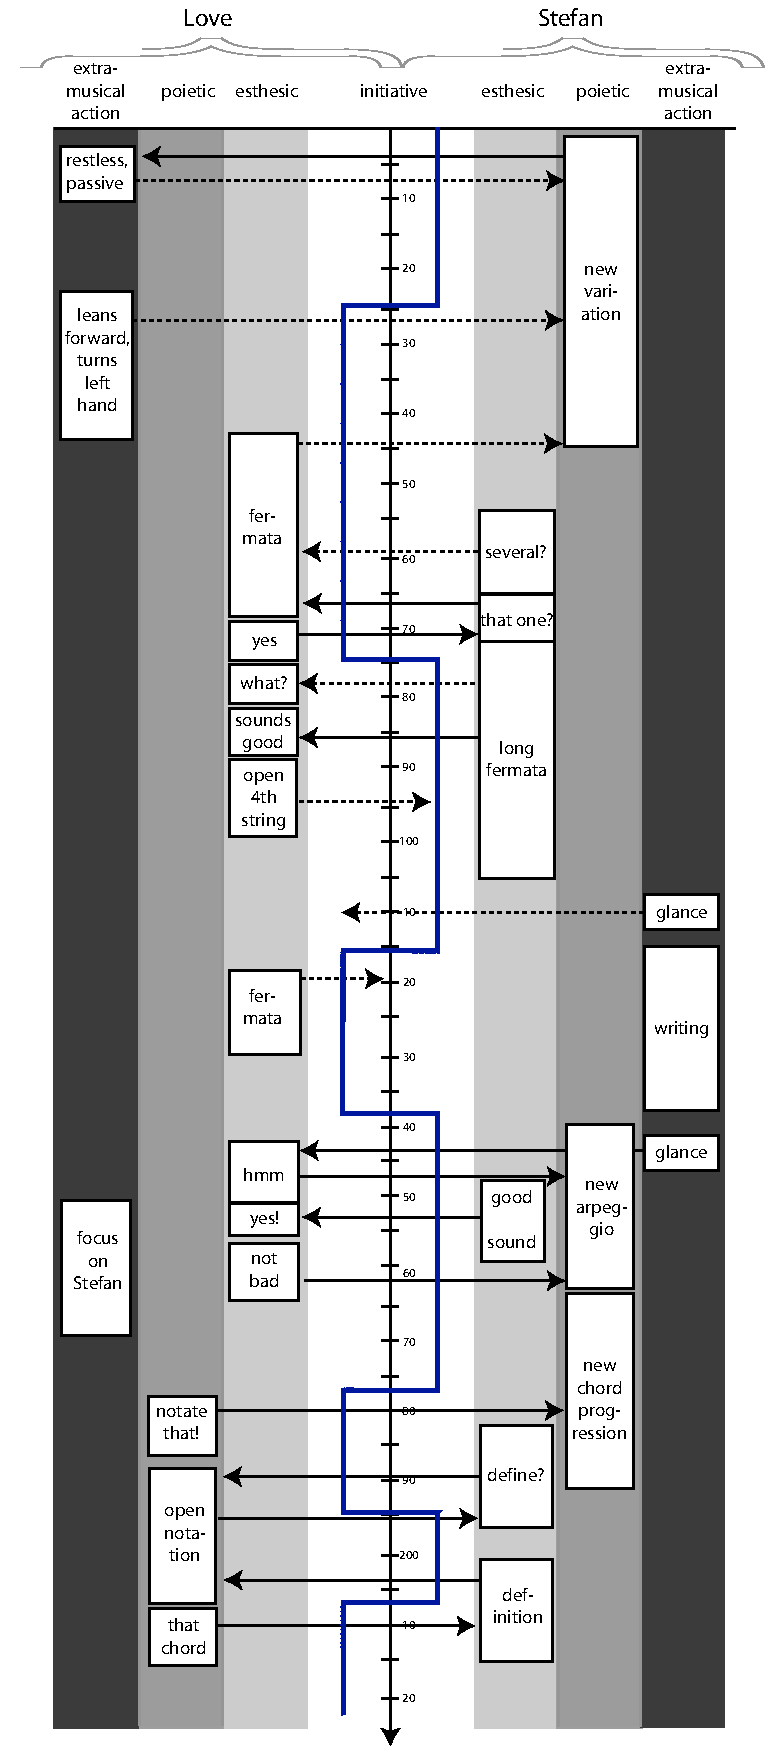
\includegraphics[width=0.2\textwidth]{img/timeline_horiz.pdf}}
	       \end{center}
              \end{minipage}
              }
      	      }
\end{slide}
%%%%%%%%%%%%%%%%%%%%%%%%%%%%%%%%%%%%%%%%%%%%%%%%%%%%%%%%%%%%%%%%%%%%

%%%%%%%%%%%%%%%%%%%%%%%%%%%%%%%%%%%%%%%%%%%%%%%%%%%%%%%%%%%%%%%%%%%%
\begin{slide}
 \section*{Computer-Musician interaction.}
  \subsection{Reflections on the results from the video analysis.}
      \liststepwise
      {
      \step
            {
	     \begin{itemize}
	      \item {Noise in communication is not a problem.}
	      \step{\item {Direction is more important than
		    synchronicity.}}
	      \step{\item {The initiative can shift independently of the
		    esthesic and poietic processes.}}
	     \end{itemize}
            }
     	      }
\end{slide}
%%%%%%%%%%%%%%%%%%%%%%%%%%%%%%%%%%%%%%%%%%%%%%%%%%%%%%%%%%%%%%%%%%%%

%%%%%%%%%%%%%%%%%%%%%%%%%%%%%%%%%%%%%%%%%%%%%%%%%%%%%%%%%%%%%%%%%%%%
\begin{slide}
 \section{Deconstructing the idea of the composer}
  \subsection{Intentionality - Creative force.}
      \liststepwise
      {
      \step
            {
              \begin{minipage}[h]{\textwidth}
	       \begin{center}
	       {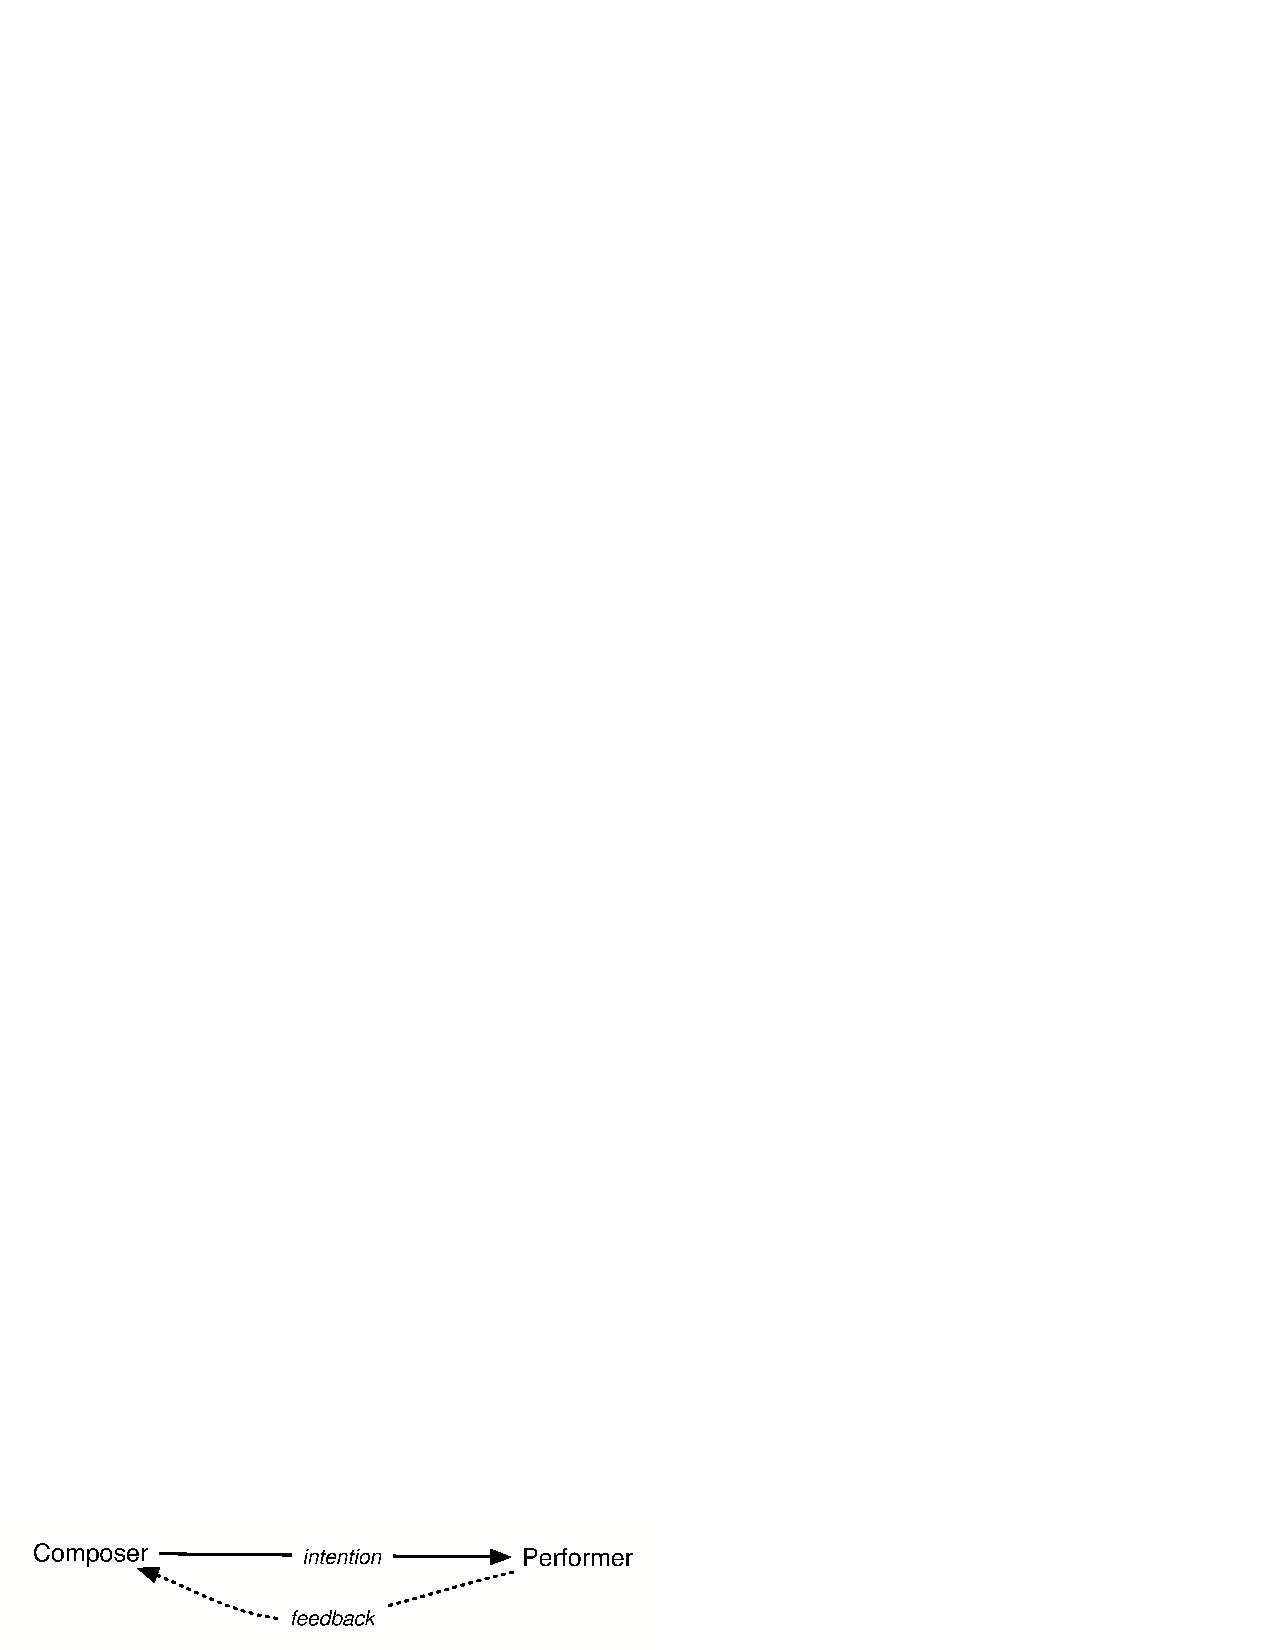
\includegraphics[]{img/composer-performer.pdf}}
	       \end{center}
              \end{minipage}
              }
      \step
            {
              \begin{minipage}[h]{\textwidth}
	       \begin{center}
	       {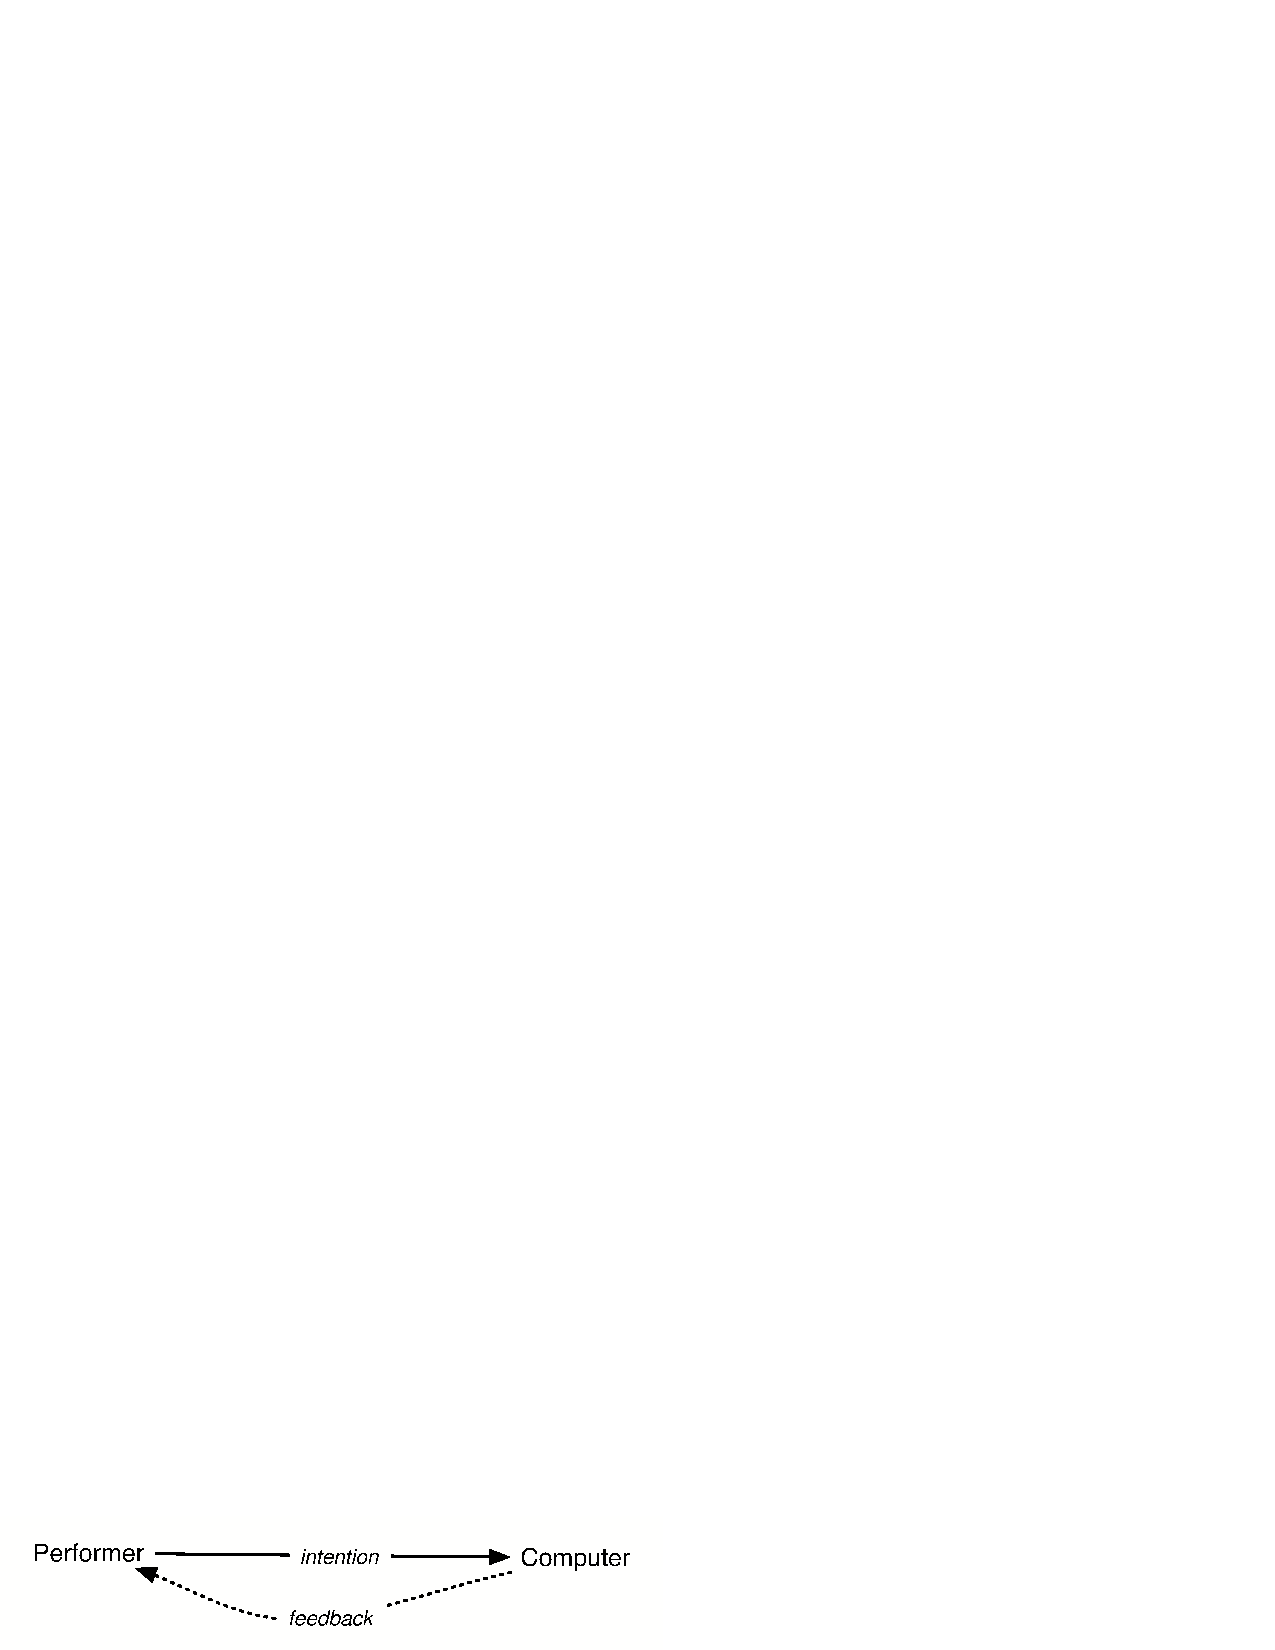
\includegraphics[]{img/performer-computer.pdf}}
	       \end{center}
              \end{minipage}
              }
     	      }
\end{slide}
%%%%%%%%%%%%%%%%%%%%%%%%%%%%%%%%%%%%%%%%%%%%%%%%%%%%%%%%%%%%%%%%%%%%

%%%%%%%%%%%%%%%%%%%%%%%%%%%%%%%%%%%%%%%%%%%%%%%%%%%%%%%%%%%%%%%%%%%%

\slidepagestyle{empty}
\begin{slide}
\bibliography{bibliography}
\bibliographystyle{apalike}
\end{slide}
%%%%%%%%%%%%%%%%%%%%%%%%%%%%%%%%%%%%%%%%%%%%%%%%%%%%%%%%%%%%%%%%%%%%
\end{document}
%%%%%%%%%%%%%%%%%%%%%%%%%%%%%%%%%%%%%%%%%%%%%%%%%%%%%%%%%%%%%%%%%%%%
%%%%%%%%%%%%%%%%%%%%%%%%%%%%%%%%%%%%%%%%%%%%%%%%%%%%%%%%%%%%%%%%%%%%


